\documentclass{standalone}
\usepackage{tikz}
\usetikzlibrary{shapes.geometric, arrows.meta, positioning}

\tikzstyle{block} = [rectangle, draw, text centered, minimum height=1cm, minimum width=4em, text width=3cm]
\tikzstyle{arrow} = [thick,->,>=stealth]
\tikzstyle{skip} = [thick, dashed,->,>=stealth]
\tikzstyle{attention} = [circle, draw, text centered, minimum height=1cm, minimum width=2em]

\begin{document}
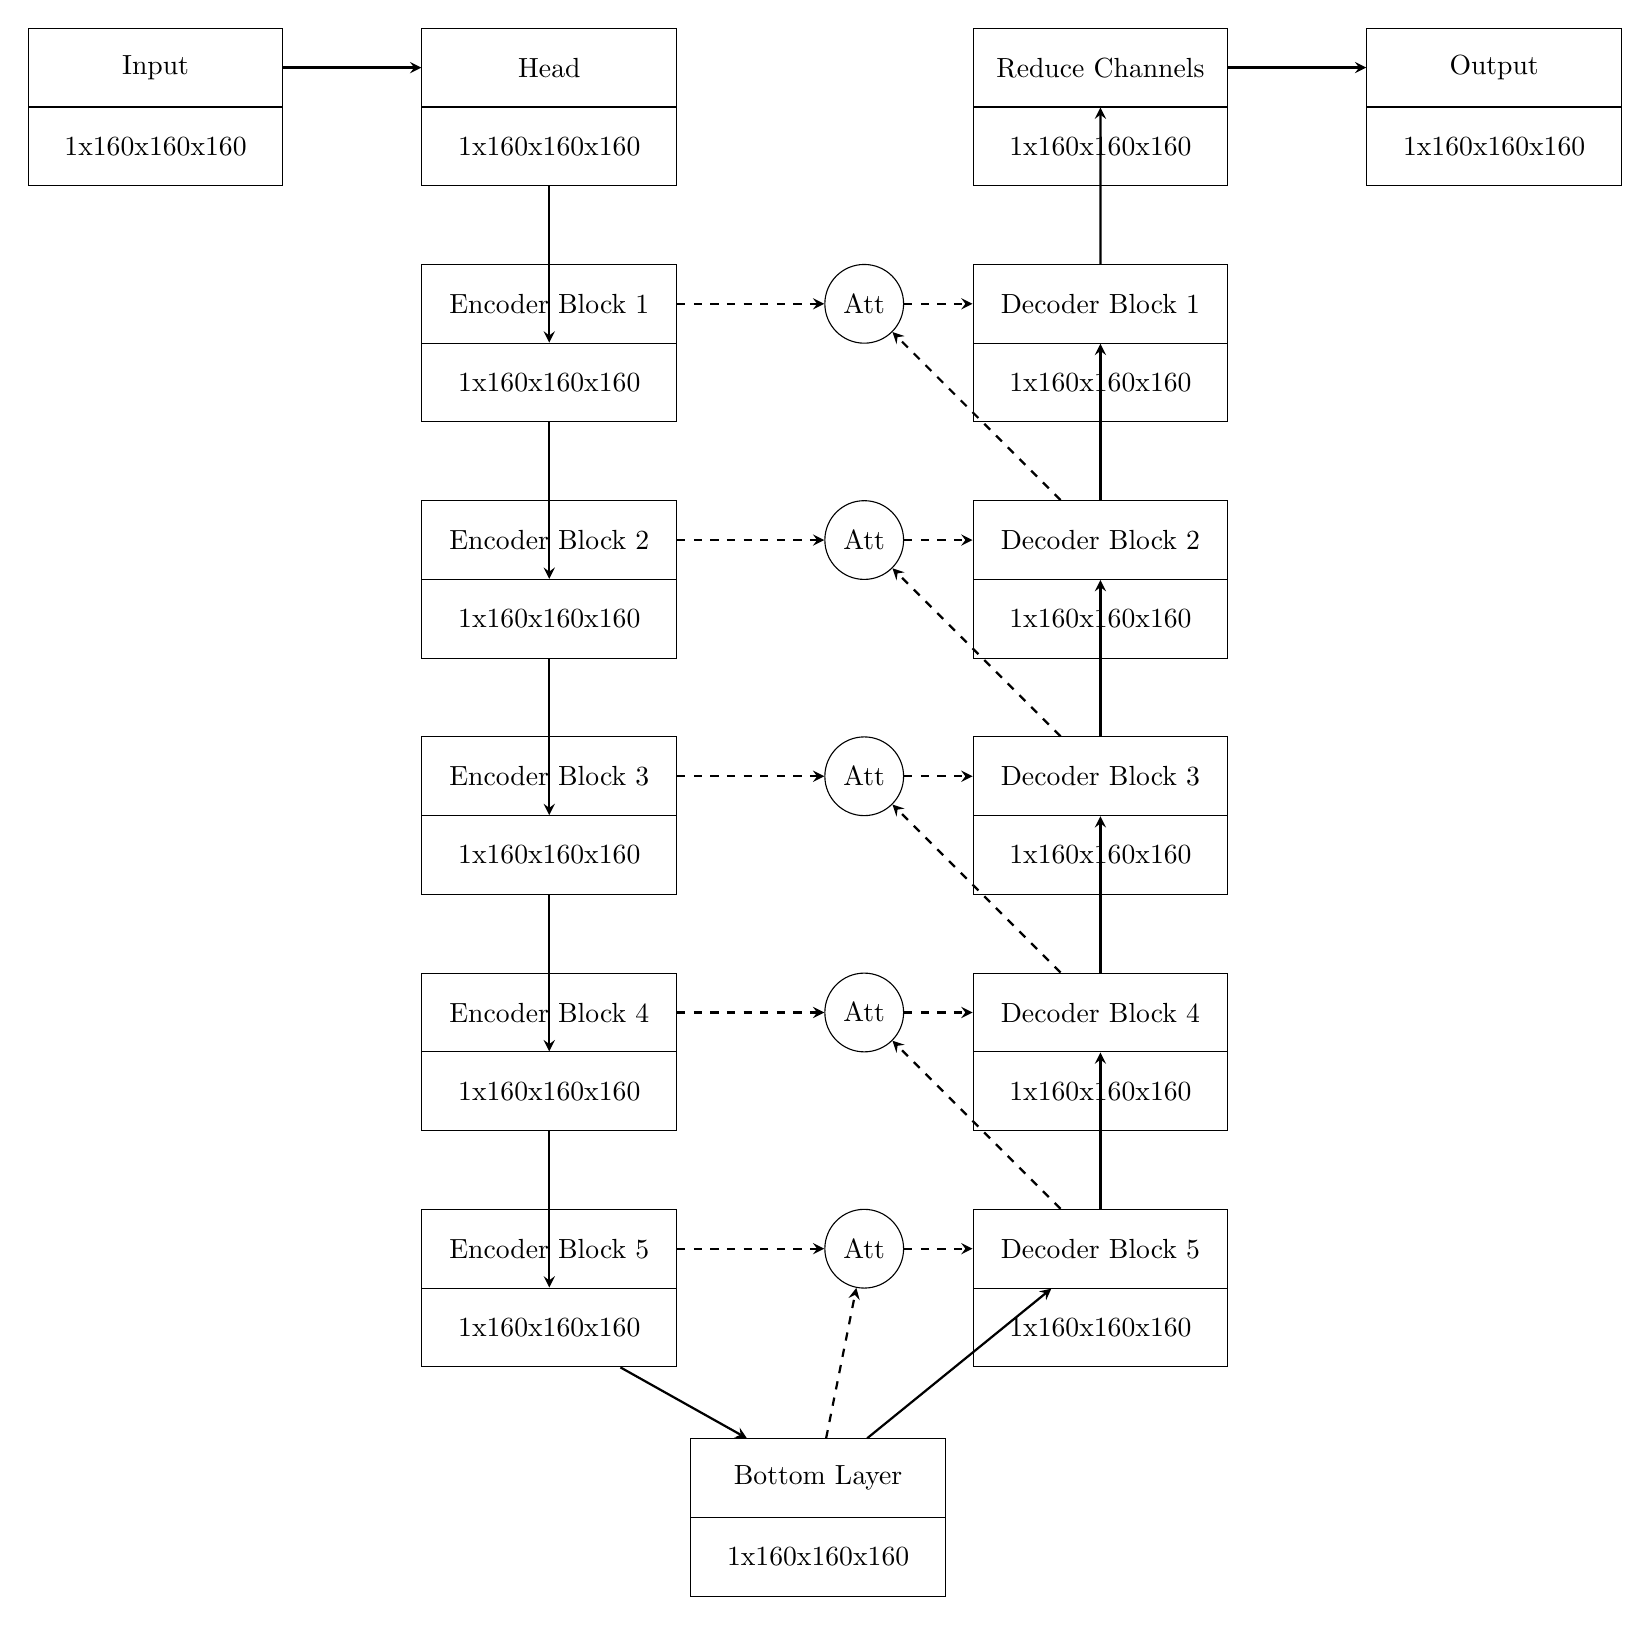
\begin{tikzpicture}[node distance=2cm]

    % Contracting path
    \node (input) [block] {Input};
    \node (input_size) [block, below of=input, yshift=1cm]{1x160x160x160};

    \node (head) [block, right of=input, xshift=3cm] {Head};
    \node (head_size) [block, below of=head, yshift=1cm]{1x160x160x160};

    \node (enc1) [block, below of=head_size] {Encoder Block 1};
    \node (enc1_size) [block, below of=enc1, yshift=1cm]{1x160x160x160};

    \node (enc2) [block, below of=enc1_size] {Encoder Block 2};
    \node (enc2_size) [block, below of=enc2, yshift=1cm]{1x160x160x160};

    \node (enc3) [block, below of=enc2_size] {Encoder Block 3};
    \node (enc3_size) [block, below of=enc3, yshift=1cm]{1x160x160x160};

    \node (enc4) [block, below of=enc3_size] {Encoder Block 4};
    \node (enc4_size) [block, below of=enc4, yshift=1cm]{1x160x160x160};

    \node (enc5) [block, below of=enc4_size] {Encoder Block 5};
    \node (enc5_size) [block, below of=enc5, yshift=1cm]{1x160x160x160};

    \node (bottom) [block, below right of=enc5_size, xshift=2cm, yshift=-0.5cm] {Bottom Layer};
    \node (bottom_size) [block, below of=bottom, yshift=1cm]{1x160x160x160};

    % Attention Mechanisms
    \node (att5) [attention, right of=enc5, xshift=2cm] {Att};
    \node (att4) [attention, right of=enc4, xshift=2cm] {Att};
    \node (att3) [attention, right of=enc3, xshift=2cm] {Att};
    \node (att2) [attention, right of=enc2, xshift=2cm] {Att};
    \node (att1) [attention, right of=enc1, xshift=2cm] {Att};

    % Expanding Path
    \node (dec5) [block, right of=att5, xshift=1cm] {Decoder Block 5};
    \node (dec5_size) [block, below of=dec5, yshift=1cm]{1x160x160x160};

    \node (dec4) [block, right of=att4, xshift=1cm] {Decoder Block 4};
    \node (dec5_size) [block, below of=dec4, yshift=1cm]{1x160x160x160};

    \node (dec3) [block, right of=att3, xshift=1cm] {Decoder Block 3};
    \node (dec5_size) [block, below of=dec3, yshift=1cm]{1x160x160x160};

    \node (dec2) [block, right of=att2, xshift=1cm] {Decoder Block 2};
    \node (dec5_size) [block, below of=dec2, yshift=1cm]{1x160x160x160};

    \node (dec1) [block, right of=att1, xshift=1cm] {Decoder Block 1};
    \node (dec5_size) [block, below of=dec1, yshift=1cm]{1x160x160x160};

    \node (reduce) [block, right of=head, xshift=5cm] {Reduce Channels};
    \node (dec5_size) [block, below of=reduce, yshift=1cm]{1x160x160x160};

    \node (output) [block, right of=reduce, xshift=3cm] {Output};
    \node (dec5_size) [block, below of=output, yshift=1cm]{1x160x160x160};

    % ==== Arrows
    % Contracting
    \draw [arrow] (input) -- (head);
    \draw [arrow] (head_size) -- (enc1_size);
    \draw [arrow] (enc1_size) -- (enc2_size);
    \draw [arrow] (enc2_size) -- (enc3_size);
    \draw [arrow] (enc3_size) -- (enc4_size);
    \draw [arrow] (enc4_size) -- (enc5_size);
    \draw [arrow] (enc5_size) -- (bottom);

    % Expanding
    \draw [arrow] (bottom) -- (dec5);
    \draw [arrow] (dec5) -- (dec4);
    \draw [arrow] (dec4) -- (dec3);
    \draw [arrow] (dec3) -- (dec2);
    \draw [arrow] (dec2) -- (dec1);
    \draw [arrow] (dec1) -- (reduce);
    \draw [arrow] (reduce) -- (output);

    % Attention
    \draw [skip] (bottom) -- (att5);
    \draw [skip] (dec5) -- (att4);
    \draw [skip] (dec4) -- (att3);
    \draw [skip] (dec3) -- (att2);
    \draw [skip] (dec2) -- (att1);

    % Skip Connections
    \draw [skip] (enc5) -- (att5);
    \draw [skip] (att5) -- (dec5);
    \draw [skip] (enc4) -- (att4);
    \draw [skip] (att4) -- (dec4);
    \draw [skip] (enc3) -- (att3);
    \draw [skip] (att3) -- (dec3);
    \draw [skip] (enc2) -- (att2);
    \draw [skip] (att2) -- (dec2);
    \draw [skip] (enc1) -- (att1);
    \draw [skip] (att1) -- (dec1);

\end{tikzpicture}
\end{document}